\chapter{Bisherige Forschung}

\lipsum[100]

\section{Kognitive Verzerrungen und implicit bias}

Unter kognitiven Verzerrungen (englisch: \emph{cognitive biases} oder \emph{cognitive illusions}) versteht man psychologische Effekte, welche zu einer Wahrnehmung oder Beurteilung führen, die von der realen Situation abweicht \citep{pohl2004cognitive}.
Die zahlreichen Manifestationen dieser Verzerrungen äußern sich auf verschiedene Art und Weise -- einen Überblick liefert \autoref{fig:cognitive-bias-cheat-sheet}.

\begin{figure}[h!]
	\centering
	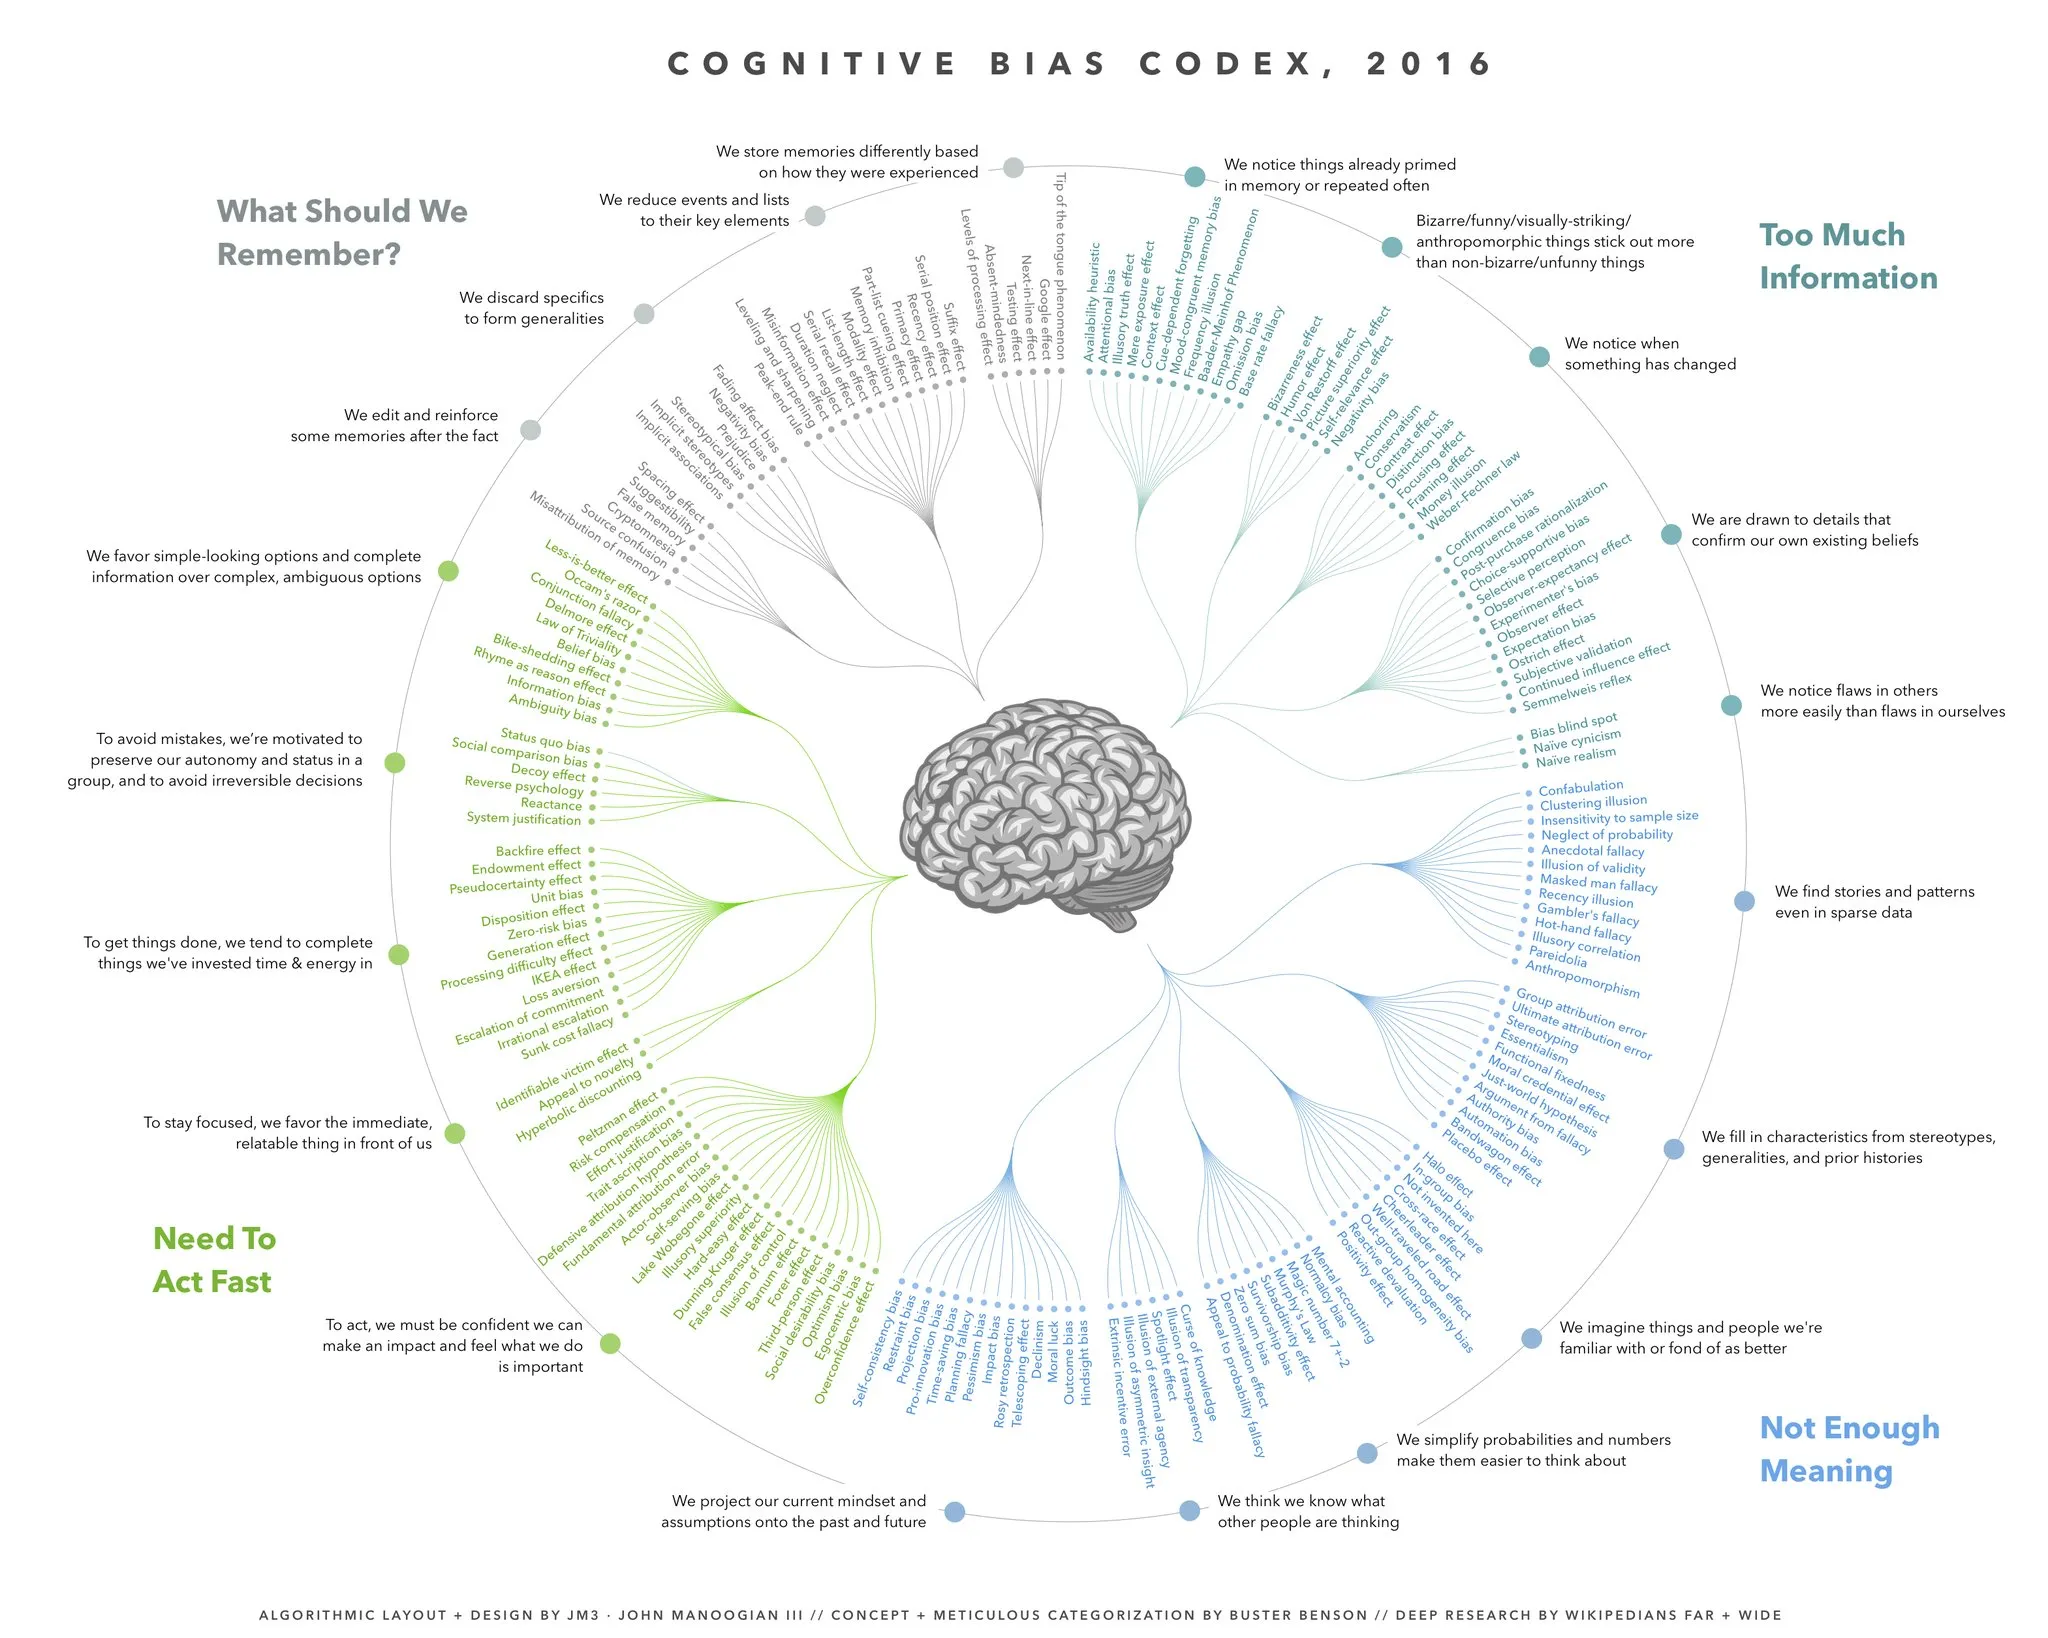
\includegraphics[width=\textwidth]{resources/cognitive-bias-cheat-sheet.png}
	\caption{Cognitive Bias Codex -- Beispiele verschiedener kognitiver Biases \citep{benson2016cognitive}}
	\label{fig:cognitive-bias-cheat-sheet}
\end{figure}

Wie in \autoref{fig:informationskreislauf} dargestellt werden bei der Integration neuer Informationen vier Phasen durchlaufen.
Aus der riesigen Menge der auf uns einströmenden Informationen werden zunächst einige wenige selektiert, aus welchen wir uns mithilfe unserer bisherigen Erinnerung einen Sinn machen können.
Unser Vorwissen wird dann genutzt, um sie in einen Kontext einzubetten, welcher anschließend unser Handeln beeinflusst.
Diese Handlungen fließen danach wiederum in unsere Erinnerung ein, auf die bei neuen Informationen zugegriffen wird.

\begin{figure}[h!]
	\centering
	\includegraphics[width=0.5\textwidth]{resources/informationskreislauf.jpg}
	\caption{Kreislauf der Integration von neuen Informationen}
	\label{fig:informationskreislauf}
\end{figure}

Bei jedem Phasenübergang finden dabei Filtereffekte statt.
Nach \cite{benson2016cognitive} kristallisieren sich dabei vier Problemstellungen heraus, mit denen das menschliche Gehirn tagtäglich konfrontiert wird.
Jede der folgenden Kategorien repräsentiert dabei einen der dargestellten Übergänge zwischen den Phasen.

\begin{enumerate}
	\item \emph{Informationsüberflutung}: Bereits seit Beginn der Existenz menschlicher Aufzeichnungen von Informationen existiert das Problem der Überflutung durch ebenjene \citep{bawden2020information}.
	Aufgrund technischer Entwicklungen und der Verbreitung des Internets hat sich die Menge an Informationen, die auf uns einwirken, insbesondere in den letzten Jahrzehnten extrem vergrößert \citep{siegler2010every}.
	So gaben 22.5\% der Deutschen im Jahr 2021 Informationsüberflutung als eine der Hauptursachen für Stress an \citep{meyer2021entspann}.
	Dies beeinflusst auch die Qualität professioneller Entscheidungen, beispielsweise im Gesundheitssystem \citep{hall2004information}, beim Management von Personal \citep{volnhals2008information} und Marketing \citep{meyer1998information} oder in der Wissenschaft \citep{landhuis2016scientific}.
	
	Nach der \emph{cognitive load theory} \citep{atkinson1968human} ist das menschliche Arbeitsgedächtnis sehr begrenzt.
	Aufgrund der übermächtigen Menge an Informationen, die auf uns einwirken, sind unsere Gehirne daher dazu gezwungen, aggressiv zu filtern \citep{savolainen2007filtering}.
	Das Resultat können fehlerhafte Schlussfolgerungen sein, beispielsweise in Form eines \emph{confirmation bias} \citep{goette2019information}.
	
	\item \emph{Mangel an Kontext}: Die Welt, in der wir leben, ist sehr komplex.
	Dennoch ist es notwendig, dass wir aus den wenigen uns gegebenen Informationen korrekte Vorhersagen treffen und ihnen eine angemessene Bedeutung zuweisen.
	Das Erkennen von Mustern trotz eines Mangels an Kontext ist in der Realität häufig unausweichlich.
	Doch gerade deshalb kann es vorkommen, dass wir eine Übergeneralisierung vornehmen und Beziehungen zwischen Informationen herstellen, obwohl diese nicht oder anders existieren.
	
	Ein Beispiel dafür ist die sogenannte \emph{Konfabulation} \citep{gilboa2002cognitive}:
	Eine Person meint, sich an ein Ereignis zu erinnern und kann konkrete Erinnerungen dazu nennen -- jedoch stellen sich diese bei Überprüfung als falsch bzw. ausgedacht heraus.
	Bekannt ist diese Art der kognitiven Verzerrung z.B. durch den \emph{Mandela-Effekt}, eine kollektive Konfabulation, nach der Nelson Mandela bereits in den 1980er-Jahren in Haft (und nicht erst 2013 in Freiheit) gestorben sei.
	Ein ähnlicher Effekt kann auch in Bezug auf visuelle Erinnerungen beobachtet werden \citep{prasad2022visual}, beispielsweise erinnern sich viele Menschen an einen Monopoly-Mann mit Monokel, obwohl dieser nie mit Monokel dargestellt worden ist.
	
	%TODO: Eventuell diesen Teil hinter die Aufzählung verschieben? Unterscheidung explicit/implicit stereotype
	Besonders relevant für diese Arbeit ist auch die Bildung von \emph{Stereotypen}.
	Dabei handelt es sich um ``weitverbreitete, jedoch feste und stark vereinfachte Bilder oder Vorstellungen zu einem bestimmten Typ von Personen oder Dingen'' \citep[Übers. d. Verf.]{bordalo2016stereotypes}. %TODO:Zitat aus Oxford Dictionary
	Insbesondere in Bezug auf die Zugehörigkeit zu ethnischen Gruppen \citep{brigham1971ethnic, guichard1977ethnic, mastro2009effects} und Geschlecht \citep{hoffman1990gender, heilman2012gender, haines2016times, ellemers2018gender} gab und gibt es immer noch viel aktuelle Forschung, da die Effekte negativer Stereotype unabhängig von gesellschaftlichen Reformen aktuell bleiben.
	
	\item \emph{Notwendigkeit, schnell zu handeln}: Trotz der Fülle an Informationen, die auf uns einströmen, dürfen wir uns nicht durch das Abwägen von Optionen aufhalten lassen, sondern müssen zuverlässig schnelle und gute Entscheidungen treffen.
	Aus diesem Grund liegt unser Fokus häufig auf den offensichtlichen und einfachen Dingen, anstatt sich in den komplizierten Details der Situation zu verlieren.
	Ein Beispiel hierfür ist der \emph{identifiable victim effect}, nach dem Menschen eher bereit sind, Ressourcen für konkrete und identifizierbare als für abstrakte, statistische Opfer bereitzustellen \citep{jenni1997explaining}.
	Weiterhin beschäftigen wir uns eher mit Trivialiäten als komplexen Problemen \citep{parkinson1958parkinson}, wie der \emph{bike shed effect} visualisiert:
	Je weniger komplex das Problem, desto mehr Zeit wird dafür aufgewendet, eine Entscheidung darüber zu treffen.
	
	Damit wir trotz des Informationsmangels nicht zögern zu handeln, überschätzen wir unsere Fähigkeiten und Urteilskraft häufig (\emph{overconfidence effect}, \cite{moore2008trouble}) und legen höheren Wert auf unsere eigene Wahrnehmung \citep{ross1979egocentric}.
	Diese Überschätzung findet insbesondere dann statt, wenn unsere tatsächliche Kompetenz relativ niedrig ist, wie der bekannte \emph{Dunning-Kruger-Effekt} \citep{dunning2011dunning} zeigt.
	
	\item \emph{Fehlbarkeit von Erinnerungen}: Nachdem wir der Informationsflut mit radikaler Filterung und Selektion begegnet sind, ihr vermeintlichen Kontext zugewiesen haben und auf Basis dieser Entscheidungen gehandelt haben, stehen wir vor einem weiteren Problem.
	Über die Nützlichkeit dieser Informationen in der Zukunft muss spekuliert werden, und so kommt es zu Verzerrungen der Realität.
\end{enumerate}


%TODO: Gründe für stereotype

Beim implicit bias (oder auch implicit stereotype) handelt es sich um ``eine Reihe von Überzeugungen über Merkmale, welche für die Mitglieder einer sozialen Kategorie charakteristisch sind'' \citep[Übers. d. Verf.]{greenwald1995implicit}.

\section{Bias Awareness}

Eine höhere Bias Awareness trägt dazu bei, den eigenen impliziten Bias zu reduzieren \citep{pope2018awareness} und hilft, den Einfluss von Biases auf beobachtete Handlungen zu erkennen \citep{perry2015modern}.

\section{Biases im schulischen Kontext}

Verzerrungen in Deutsch und Mathematik bei Grundschullehrkräften: \cite{lorenz2016stereotype}

Hintergrundmerkmale $\rightarrow$ Lehrkrafteinschätzung Motivation $\rightarrow$ Lehrkrafterwartungen Leistungen: Soziale und geschlechtsbezogene Verzerrungen, ethnischer Hintergrund jedoch unabhängig von Lehrkrafteinschätzung Motivation \cite{gentrup2020einschatzungen}